\section{Environmental Configuration}
\subsection{Overview}

PyTorch and TensorFlow are two of the most popular deep learning frameworks used for building and training machine learning models. When setting up a development environment for working with these frameworks, having a Linux native environment or WSL2 (Windows Subsystem for Linux) can significantly ease the configuration process and subsequent usage with GPU acceleration, provided available Nivdia hardware. You can confirm your system hardware supports CUDA and cuDNN \href{https://developer.nvidia.com/cuda-gpus}{here}. Both PyTorch and TensorFlow offer GPU support, which allows for faster training times.

A Linux native environment or WSL2 is advantageous for configuring a machine learning environment in Python due to better package compatibility, efficient package managers, robust command-line tools, improved GPU support, enhanced reproducibility, and alignment with the machine learning community's practices.

\subsection{Windows Subsystem for Linux}
This section will breifly walk through how to install and enable WSL2 for your windows machine, documentation found \href{https://learn.microsoft.com/en-us/windows/wsl/install}{here}.
\begin{itemize}
	\item Launch PowerShell or Windows Command Prompt as an administrator by right-clicking and choosing "Run as administrator." then enable the usage of WSL and virtual enviroments by entering 
	\begin{lstlisting}[language=bash]
		Enable-WindowsOptionalFeature -Online -FeatureName Microsoft-Windows-Subsystem-Linux
		Enable-WindowsOptionalFeature -Online -FeatureName VirtualMachinePlatform\end{lstlisting}
	\item Next either download WSL from the window store or input the command
	 \begin{lstlisting}[language=bash]
	 	wsl --install\end{lstlisting} and then reboot your machine to complete the installation process.
	\item After the restart, open the Microsoft Store and search "Linux." You'll find various Linux distributions available. Choose the one that supports your intended version of CUDA refrenced below.
	\item After the installation is finished, launch the distribution from the Start menu or by searching for its name. The first time You run the Linux distribution, you will be prompted to set up a new Linux user and password.
	\item Configure your default linux distrobution to the installed distrobution using the powershell command \begin{lstlisting}[language=bash]
		wsl -s <DistributionName>\end{lstlisting}
\end{itemize}

You may now execute commands from Powershell to run in your install linux distrobution using the command "wsl" or "bash" to enter linux terminal.

\subsection{Linux Python Environment Management}

Before installing PyEnv, found \href{https://github.com/pyenv/pyenv}{here}, make sure you have the necessary dependencies in your WSL environment:
\begin{itemize}
	\item From bash within wsl run these commands
	\begin{lstlisting}[language=bash]
		sudo apt update
		sudo apt install -y git curl make build-essential libssl-dev zlib1g-dev libbz2-dev libreadline-dev libsqlite3-dev wget llvm libncurses5-dev xz-utils tk-dev libxml2-dev libxmlsec1-dev libffi-dev liblzma-dev \end{lstlisting}

	\item Next you may install PyEnv using curl
	\begin{lstlisting}[language=bash]
		curl https://pyenv.run | bash \end{lstlisting}
	
	\item Next you must add PyEnv to the Path environment variable using the following commands
	\begin{lstlisting}[language=bash]
		export PYENV_ROOT="$HOME/.pyenv"
		export PATH="$PYENV_ROOT/bin:$PATH"
		eval "$(pyenv init --path)"
		source ~/.bashrc \end{lstlisting}
	\item You may now install and manage multiple python enviroments separate from your Linux system Python environment using the follow commands:
	\begin{itemize}
		\item to list available Python versions
		\begin{lstlisting}[language=bash]
			pyenv install --list \end{lstlisting}
		\item to list install a Python version
		\begin{lstlisting}[language=bash]
			pyenv install <VERSION NUM> \end{lstlisting}
		\item to set the PyEnv virtual environment as the primary Python in enviroment 
		\begin{lstlisting}[language=bash]
			pyenv global <VERSION NUM> \end{lstlisting}
	\end{itemize}

\end{itemize}

\subsection{GPU configuration}

\begin{wrapfigure}{r}{0.5\textwidth}
	\vspace{-1.5cm}
	\begin{center}
		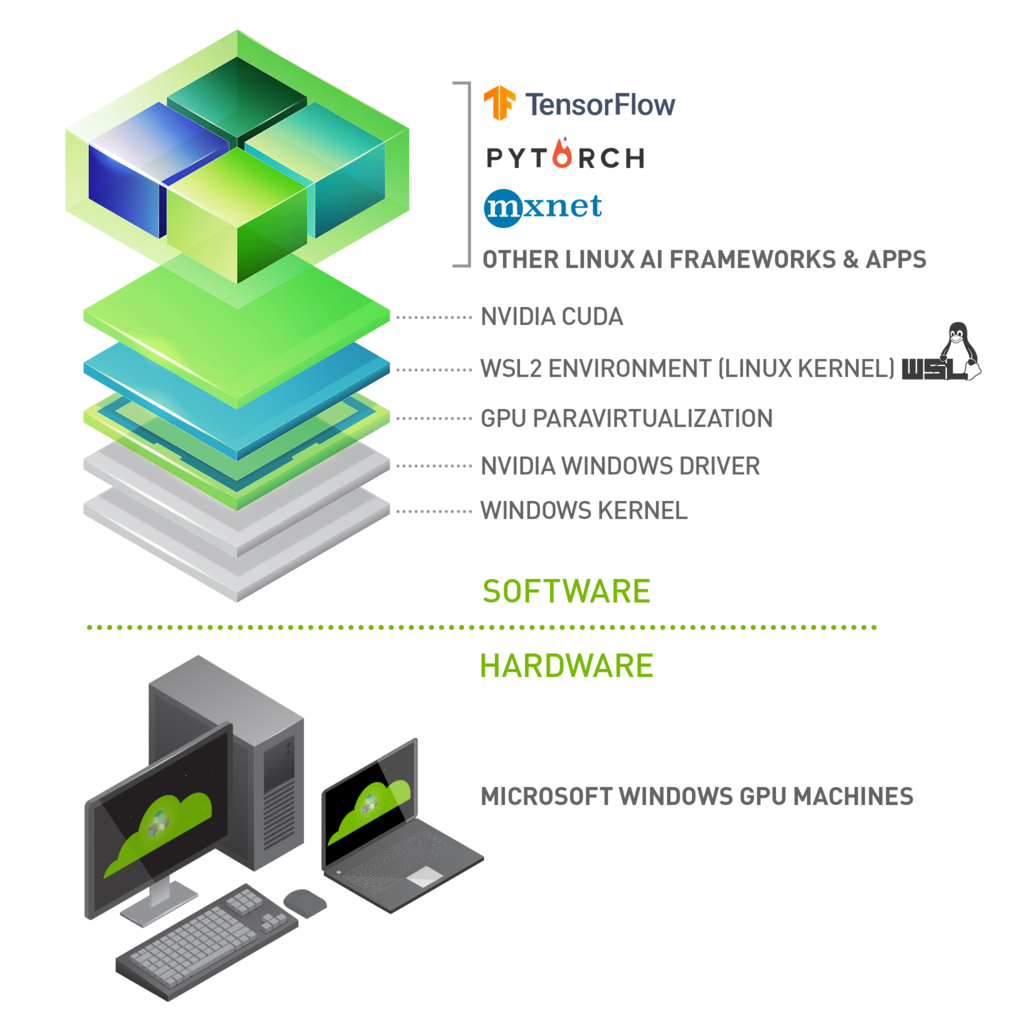
\includegraphics[width=.48\textwidth]{wsl-launch-upt-0625-rz.png}
	\end{center}
	\label{fig:arch}
\end{wrapfigure}

Now supported in WSL2, available for Window 10 and 11, and the Linux OS natively CUDA and cuDNN for running machine learning applications such a TensorFlow and PyTorch. Following the guidance available from Nvidia \href{https://docs.nvidia.com/cuda/wsl-user-guide/index.html}{here} the current release WSL 2 v1.2.5, released April 20, 2023, supported by Windows 10 and 11, uses a paravirtualizationShown in Fig.\ref{fig:arch} of the GPU architecture for the Linux subsystem to interact directly with the Window GPU driver. Whether using WSL2 as outlines in this guide or native linux installations the drivers can be found available from Nvidia \href{https://www.nvidia.com/Download/index.aspx?lang=en-us}{here} to enable the usage of CUDA and cuDNN for machine learning applications.

\pagebreak
\subsection{Environmental Configurations}
Detailed here is the environments used in this study, attached in the github :
\subsubsection{TensorFlow V1.X}
\begin{itemize}
	\item \textit{Python Version} == 3.6.x
	\item to install using pip
	\begin{lstlisting}[language=bash]
		pip install -r requirements.txt \end{lstlisting}
	\item to set the PyEnv virtual environment as the primary Python in enviroment 
	\begin{lstlisting}[language=bash]
		tensorflow-gpu==1.15
		dm-sonnet==1.36\end{lstlisting}
\end{itemize}
\subsubsection{PyTorch}
\begin{itemize}
	\item \textit{Python Version} == 3.10.x
	\item to install using pip
	\begin{lstlisting}[language=bash]
		pip install -r requirements.txt \end{lstlisting}
	\item to set the PyEnv virtual environment as the primary Python in enviroment 
	\begin{lstlisting}[language=bash]
		tensorflow-gpu>=1.15,<2
		dm-sonnet<2
		matplotlib
		absl-py
		numpy\end{lstlisting}
\end{itemize}


